\chapter{Metodología de desarrollo}\label{chap:metodologia}

El desarrollo organiza el prototipo en incrementos verificables. La descripción distingue arquitectura, código disponible y criterios de aceptación, de modo que un componente diseñado o una captura de pantalla se distingan de una validación.

\section{Organización del trabajo}\label{sec:planificacion}

El equipo, de dos integrantes, adopta Scrum como marco de trabajo y lo complementa con un tablero Kanban \parencite{ScrumGuide2020,Anderson2010}. Scrum aporta el ritmo: sprints de dos semanas con un objetivo acordado y un incremento revisable al cierre. Kanban aporta la visibilidad del flujo: cada tarea de investigación, diseño, implementación o redacción pasa por las columnas Pendiente, En curso, En revisión y Hecho, con un límite de dos tareas en curso por integrante. La elección responde a tres condiciones del Proyecto. Los requerimientos se precisan a medida que avanza la investigación con usuarios. El plazo acotado exige incrementos evaluables en fechas fijas. Un equipo de dos personas no admite la estructura completa de roles de Scrum, de modo que ambos integrantes comparten las responsabilidades de producto y de desarrollo, y el tutor actúa como interesado en la revisión de cada incremento.

El trabajo se organiza en investigación, especificación, diseño, construcción de módulos, integración y evaluación. Cada etapa produce un resultado distinto: bibliografía e instrumentos de investigación, requerimientos, diagramas, código y registros de pruebas. El código se verifica con pruebas funcionales; la utilidad para el usuario, con sesiones de evaluación.

\subsection{Eventos, artefactos y herramientas}\label{subsec:scrum-eventos}

Cada sprint comienza con una planificación en la que se fija el objetivo y se seleccionan historias del backlog. La sincronización diaria es asíncrona, por mensajes, con una reunión breve semanal. Al cierre se revisa el incremento entre los integrantes y, al completar cada etapa, con el tutor; la retrospectiva registra qué ajustar en el sprint siguiente. El backlog de producto reúne los requerimientos de las Subsecciones~\ref{sec:req-funcionales} y~\ref{sec:req-no-funcionales} descompuestos en historias de usuario; el backlog del sprint es el conjunto de tarjetas del tablero. Un incremento se considera terminado cuando el código tiene pruebas que pasan en la integración continua, la solicitud de incorporación fue revisada por el otro integrante y la sección correspondiente del Proyecto está actualizada.

El tablero se lleva en GitHub Projects, asociado a los repositorios del Proyecto y de la aplicación; las ramas y solicitudes de incorporación registran el trabajo de cada historia. La Figura~\ref{fig:kanban} muestra el estado del tablero al cierre del sprint 16.
% Tablero Kanban del Proyecto (GitHub Projects), estado al 22 de octubre de 2026.
\begin{figure}[ht]\centering
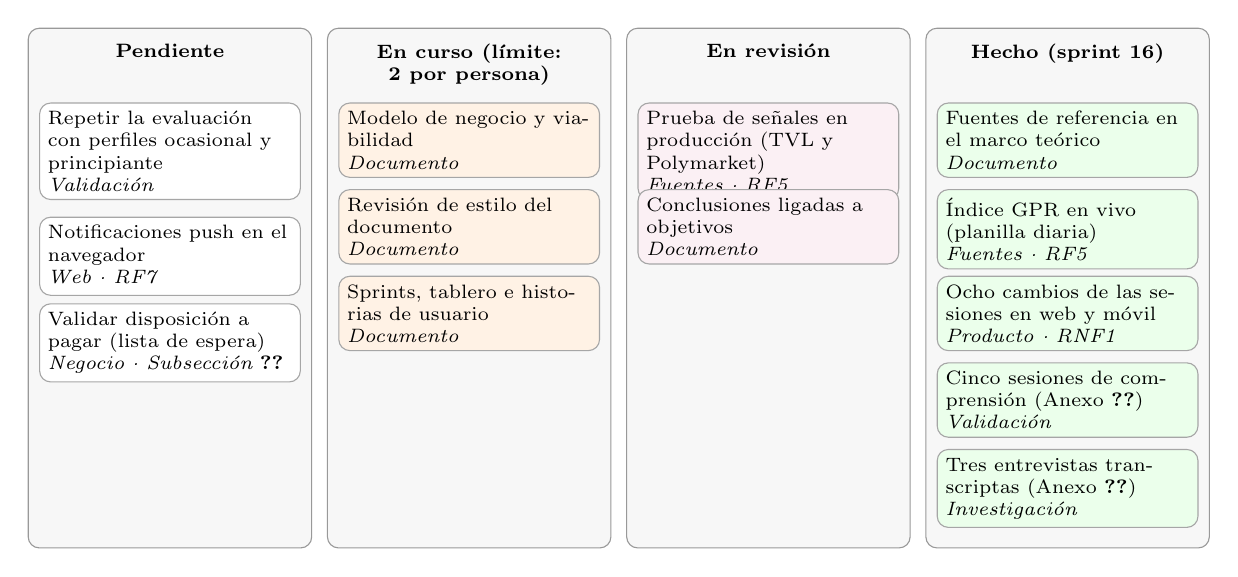
\begin{tikzpicture}[font=\scriptsize,
  col/.style={draw=black!40,rounded corners,fill=black!3,minimum width=3.6cm,minimum height=6.6cm,anchor=north},
  hdr/.style={font=\scriptsize\bfseries,anchor=north},
  card/.style={draw=black!35,rounded corners,fill=white,text width=3.1cm,align=left,inner sep=3pt,anchor=north},
  done/.style={card,fill=green!8},rev/.style={card,fill=purple!6},wip/.style={card,fill=orange!10}]
\foreach \x/\n in {0/Pendiente,3.8/En curso (límite: 2 por persona),7.6/En revisión,11.4/Hecho (sprint 16)}{
  \node[col] at (\x,0) {};\node[hdr,text width=3.3cm,align=center] at (\x,-0.08) {\n};}
% Pendiente
\node[card] (p3) at (0,-0.95) {Repetir la evaluación con perfiles ocasional y principiante\\\textit{Validación}};
\node[card] (p5) at (0,-2.4) {Notificaciones push en el navegador\\\textit{Web · RF7}};
\node[card] (p6) at (0,-3.5) {Validar disposición a pagar (lista de espera)\\\textit{Negocio · Subsección~\ref{sec:viabilidad}}};
% En curso
\node[wip] at (3.8,-0.95) {Modelo de negocio y viabilidad\\\textit{Documento}};
\node[wip] at (3.8,-2.05) {Revisión de estilo del documento\\\textit{Documento}};
\node[wip] at (3.8,-3.15) {Sprints, tablero e historias de usuario\\\textit{Documento}};
% En revisión
\node[rev] at (7.6,-0.95) {Prueba de señales en producción (TVL y Polymarket)\\\textit{Fuentes · RF5}};
\node[rev] at (7.6,-2.05) {Conclusiones ligadas a objetivos\\\textit{Documento}};
% Hecho
\node[done] at (11.4,-0.95) {Fuentes de referencia en el marco teórico\\\textit{Documento}};
\node[done] at (11.4,-2.05) {Índice GPR en vivo (planilla diaria)\\\textit{Fuentes · RF5}};
\node[done] at (11.4,-3.15) {Ocho cambios de las sesiones en web y móvil\\\textit{Producto · RNF1}};
\node[done] at (11.4,-4.25) {Cinco sesiones de comprensión (Anexo~\ref{annex:protocolo-usuarios})\\\textit{Validación}};
\node[done] at (11.4,-5.35) {Tres entrevistas transcriptas (Anexo~\ref{annex:entrevistas})\\\textit{Investigación}};
\end{tikzpicture}
\caption{Tablero Kanban del Proyecto al 23 de octubre de 2026, cierre del sprint 16. Fuente: elaboración propia a partir de GitHub Projects.}\label{fig:kanban}
\end{figure}


\subsection{Historias de usuario}\label{subsec:historias}

Las historias se redactan desde las tres personas usuarias de la Subsubsección~\ref{subsec:user-persona} y se vinculan con los requerimientos. La Tabla~\ref{tab:historias} muestra las principales y el sprint en que se completaron.
\begin{table}[ht]
\centering\small\renewcommand{\arraystretch}{1.15}
\caption{Historias de usuario principales. Fuente: elaboración propia.}\label{tab:historias}
\begin{tabular}{>{\raggedright\arraybackslash}p{1.1cm}>{\raggedright\arraybackslash}p{8.6cm}>{\raggedright\arraybackslash}p{1.6cm}>{\raggedright\arraybackslash}p{1.5cm}}\hline
\textbf{Id} & \textbf{Historia} & \textbf{Requer.} & \textbf{Sprint}\\\hline
HU01 & Como inversor activo, quiero cargar mis posiciones por ticker y cantidad para ver toda mi cartera en un solo lugar. & RF2, RF3 & 11\\
HU02 & Como inversor activo, quiero ver la exposición por clase, sector, región y moneda y el nivel de concentración para saber de qué depende mi cartera. & RF4 & 11\\
HU03 & Como inversor ocasional, quiero abrir el porqué de una observación para entender qué dato y qué regla la generaron. & RF6 & 11\\
HU04 & Como inversor activo, quiero ver señales de contexto con su fuente y su fecha para distinguir un dato vigente de uno de demostración. & RF5 & 11, 15\\
HU05 & Como persona que empieza, quiero crear una cuenta y que mis posiciones queden guardadas para no volver a cargarlas. & RF1 & 12\\
HU06 & Como usuario, quiero usar la misma cuenta desde la web y desde el teléfono para elegir el dispositivo según la ocasión. & RF7 & 15\\
HU07 & Como usuario, quiero eliminar mi cuenta y mis datos con una confirmación para controlar mi información. & RF9, RF10 & 15\\
HU08 & Como inversor activo, quiero un informe por activo con fuentes citadas para contrastar lo que leo en otros medios. & RF11 & 15\\
HU09 & Como inversor activo, quiero seguir activos que no tengo y recibir avisos con condiciones para evaluar alternativas sin mezclarlas con mi cartera. & RF12 & 16\\\hline
\end{tabular}
\end{table}

\subsection{Sprints}\label{subsec:sprints}

La Tabla~\ref{tab:sprints} reconstruye los sprints a partir del tablero y del historial de los repositorios.
\begin{table}[ht]
\centering\small\renewcommand{\arraystretch}{1.12}
\caption{Sprints del Proyecto (dos semanas cada uno). Fuente: elaboración propia.}\label{tab:sprints}
\begin{tabular}{>{\raggedright\arraybackslash}p{1.1cm}>{\raggedright\arraybackslash}p{2.4cm}>{\raggedright\arraybackslash}p{5.9cm}>{\raggedright\arraybackslash}p{3.6cm}}\hline
\textbf{Sprint} & \textbf{Fechas (2026)} & \textbf{Objetivo} & \textbf{Resultado o hito}\\\hline
1--3 & 16/3 a 26/4 & Definir tema, problema y alcance; relevar herramientas existentes. & Tema, problema y alcance definidos.\\
4--5 & 27/4 a 24/5 & Marco teórico inicial; diseño y lanzamiento de la encuesta. & Encuesta abierta el 24/5.\\
6--7 & 25/5 a 21/6 & Análisis de las primeras respuestas; estructura del documento. & Estructura del documento definida.\\
8--10 & 22/6 a 2/8 & Entrevistas, personas usuarias, arquitectura y wireframes; reglas del motor. & Diseño de Allocia con identidad visual y paleta.\\
11 & 3/8 a 16/8 & Prototipo: API, catálogo, cálculo, observaciones, cliente móvil y web (HU01 a HU04). & Encuesta cerrada el 14/8 con 190 respuestas; primer despliegue en Railway (15/8).\\
12 & 17/8 a 30/8 & Cuentas y sesión (HU05); demostración del prototipo. & Prototipo con cuentas demostrado (22/8).\\
13--14 & 31/8 a 27/9 & Reorganización del marco teórico y de los anexos. & Documento reestructurado.\\
15 & 28/9 a 11/10 & Cuenta compartida web y móvil, cifrado, correo, informes por activo (HU06 a HU08); pruebas de seguridad e integración. & 62 comprobaciones de la evaluación inicial; revisión del 10/10.\\
16 & 12/10 a 25/10 & Oportunidades (HU09); reverificación; índice GPR en vivo; infografías y modelo de negocio; tres entrevistas transcriptas; cinco sesiones de comprensión y cambios derivados. & Reverificación del 13/10; entrevistas del 22/10; sesiones del 21 al 23/10 (criterio no alcanzado: 2 de 5); ocho cambios e índice GPR desplegados (23/10).\\
17--18 & 26/10 a 22/11 & Consolidación de la evidencia y revisión final del documento. & Documento final.\\\hline
\end{tabular}
\end{table}

\section{Definición del MVP}\label{sec:mvp}

El MVP comprende carga manual, clasificación, composición, concentración y observaciones con evidencia, accesibles desde los clientes web y móvil con una misma cuenta. La integración de contexto distingue señales externas de ejemplos locales. La hipótesis de utilidad se evalúa por la comprensión de una observación y la ejecución de tareas, no por el interés declarado en la encuesta.

Los criterios técnicos se especifican en los requerimientos. Para la evaluación exploratoria de utilidad se propone que al menos cuatro de cinco participantes puedan identificar la causa de una observación y la fuente que la respalda, sin ayuda. El protocolo registra tarea, resultado, errores y comentarios. Las sesiones del 21 al 23 de octubre arrojaron dos de cinco (Subsección~\ref{sec:pruebas-usabilidad}): el umbral no se alcanzó y motivó ocho cambios de presentación, implementados y desplegados el 23 de octubre.

\section{Diseño del sistema}\label{sec:diseno}

La solución separa datos ingresados, métricas derivadas y contexto externo. Las reglas consumen esos datos sin modificar las posiciones. Cada observación lleva su evidencia y la condición que la activó, de modo que el usuario puede revisar qué parte depende de su cartera y qué parte de una señal o supuesto. Las decisiones de diseño que se apoyan en el marco teórico son las siguientes:
\begin{itemize}
\item Allocia instrumenta las etapas de monitoreo, análisis de composición y reporte del proceso de gestión de portafolios para un inversor minorista que opera sin un asesor profesional; no redacta una política de inversión ni selecciona títulos (Subsubsección~\ref{subsec:portafolios-diversificacion}).
\item Opera sobre la cartera efectivamente implementada y no prescribe pesos óptimos: la sensibilidad de la optimización media-varianza a los datos de entrada y su tendencia a concentrar la asignación fundamentan generar observaciones basadas en reglas con evidencia trazable. Señala desvíos de concentración, pero no calcula bandas de rebalanceo.
\item La relación entre un evento y una exposición se expresa mediante una regla explícita y se interpreta como una hipótesis, no como una estimación causal (Subsubsección~\ref{subsec:riesgo-geopolitico}).
\item La exposición a stablecoins se trata como una categoría propia por los riesgos descriptos para las economías emergentes (Subsubsección~\ref{subsec:tendencias}), y las probabilidades de los mercados de predicción se usan como contexto, sin recomendar operar en esas plataformas.
\item La explicación de las observaciones se apoya en la trazabilidad de las reglas; los informes redactados con un modelo de lenguaje se acotan mediante validación de esquema y de citas (Subsección~\ref{sec:seguridad}).
\end{itemize}


\section{Arquitectura de la solución}\label{sec:arquitectura}

La arquitectura se describe en tres vistas complementarias: la funcional, que asigna responsabilidades a los módulos; la técnica, que ubica esos módulos en los componentes desplegados, y la de datos, que define las entidades persistidas y sus relaciones. Cada vista se acompaña de su diagrama.

\subsection{Arquitectura funcional}\label{subsec:arq-funcional}

Los módulos de identidad, portafolio, catálogo, análisis, señales, observaciones, informes y presentación se corresponden con las responsabilidades definidas en la Subsección~\ref{sec:modulos}. El catálogo clasifica las posiciones; el análisis calcula pesos y exposiciones; las señales aportan contexto; el motor de reglas produce observaciones. Los informes por activo, redactados con un modelo de lenguaje, se apoyan en fuentes públicas y no reciben datos de la cartera. La Figura~\ref{fig:diag-funcional} representa ese recorrido.
\begin{figure}[ht]\centering
\begin{tikzpicture}[node distance=0.65cm,box/.style={draw,rounded corners,fill=blue!6,text width=8cm,align=center,minimum height=0.8cm},arr/.style={-{Stealth},thick}]
\node[box] (id) {Identidad y autorización};
\node[box,below=of id] (p) {Posiciones propias y catálogo de clasificación};
\node[box,below=of p] (a) {Cálculo de pesos, exposiciones y concentración};
\node[box,below=of a,fill=orange!8] (s) {Reglas y señales con procedencia explícita};
\node[box,below=of s,fill=green!8] (o) {Observaciones, evidencia y escenarios};
\node[box,below=of o] (c) {Presentación web y móvil};
\node[box,right=0.9cm of s,text width=4.6cm,fill=purple!8] (inf) {Informes por activo con\\modelo de lenguaje y\\citas validadas};
\foreach \x/\y in {id/p,p/a,a/s,s/o,o/c}\draw[arr] (\x)--(\y);
\draw[arr] (s.east)--(inf.west);
\draw[arr] (inf.south)|-(c.east);
\end{tikzpicture}
\caption{Organización funcional de Allocia. Fuente: elaboración propia.}\label{fig:diag-funcional}
\end{figure}


\subsection{Arquitectura técnica}\label{subsec:arq-tecnica}

La API NestJS concentra la lógica de negocio y expone contratos JSON a los clientes web y móvil. PostgreSQL almacena usuarios, instrumentos y posiciones. Redis guarda las señales en caché durante 15 minutos; fuera de producción, el código usa memoria local cuando Redis no está disponible. Ese tiempo de vida acota la reutilización de la respuesta y es independiente de la antigüedad de cada dato de origen.

La Figura~\ref{fig:diag-componentes} distingue clientes, API, persistencia y proveedores. El cliente web se despliega en Vercel; la API, el proceso de análisis y PostgreSQL, en Railway; el cliente móvil se empaqueta con EAS Build. La Subsección~\ref{sec:validacion-publicada} documenta la verificación del servicio publicado; el cifrado en reposo del proveedor de base de datos, la distribución de instaladores móviles y las pruebas completas en dispositivos quedan fuera de esa verificación.
\begin{figure}[ht]\centering
\begin{tikzpicture}[node distance=0.8cm and 0.7cm,box/.style={draw,rounded corners,fill=blue!6,text width=4.2cm,align=center,minimum height=1cm,font=\footnotesize},arr/.style={-{Stealth},thick}]
\node[box] (clients) {Web: Next.js (Vercel)\\Móvil: React Native / Expo};
\node[box,right=1.6cm of clients] (api) {API NestJS (Railway)\\Autenticación y lógica\\de negocio; proceso\\de análisis};
\node[box,right=of api,fill=purple!8] (llm) {Anthropic\\Modelo de lenguaje para\\los informes por activo};
\node[box,below=of clients,fill=teal!8] (db) {PostgreSQL\\Usuarios, catálogo\\y posiciones};
\node[box,below=of api,fill=teal!8] (caché) {Caché Redis\\Alternativa en memoria fuera de producción};
\node[box,below=of llm,fill=orange!8] (prov) {Fuentes de análisis\\Finnhub, CoinGecko,\\FRED y noticias};
\node[box,below=of db,fill=orange!8] (live) {Consultas externas\\Alternative.me, CoinGecko, DefiLlama,\\Polymarket e índice GPR (planilla diaria)};
\node[box,below=of caché,fill=orange!8] (local) {Datos locales de demostración\\(solo en desarrollo; no se publican)};
\draw[arr] (clients)--node[above,font=\scriptsize]{JSON / token}(api);
\draw[arr] (api)--(llm);
\draw[arr] (api)--(db);
\draw[arr] (api)--(caché);
\draw[arr] (live)--(caché);
\draw[arr] (local)--(caché);
\draw[arr] (prov)--(llm);
\end{tikzpicture}
\caption{Componentes y procedencia de las señales. Fuente: elaboración propia.}\label{fig:diag-componentes}
\end{figure}


\subsection{Arquitectura de datos}\label{subsec:arq-datos}

El catálogo relaciona cada ticker con nombre, clase, sector, región, moneda y precio de referencia. Una posición almacena cantidad cifrada, ticker y propietario. La entidad de usuarios registra nombre, correo, hash de contraseña, versión de sesión, preferencia de alertas y aceptación de privacidad. La persistencia agrega ejecuciones regionales, informes públicos por activo, alertas por usuario, dispositivos y un outbox para entrega push.

La relación \texttt{positions.userId} es obligatoria y declara una clave foránea a usuarios con eliminación en cascada. Las consultas privadas filtran por el propietario y la base impide posiciones huérfanas. Los casos IT06, IT10 e IT12 verifican estos comportamientos en PostgreSQL aislado. Antes de aplicar el esquema a una base preexistente hay que revisar los registros sin propietario; la evaluación no modifica bases del usuario. Las observaciones se calculan en cada consulta y no se persisten. La Figura~\ref{fig:diag-er} resume las entidades y la relación de propiedad entre usuarios y posiciones.
\begin{figure}[ht]\centering
\begin{tikzpicture}[node distance=1cm and 0.8cm,box/.style={draw,rounded corners,fill=teal!7,text width=4.4cm,align=left,inner sep=8pt,font=\small},arr/.style={-{Stealth},thick}]
\node[box] (users) {\textbf{users}\\id (PK)\\name, email\\passwordHash\\versión de sesión\\preferencia de alertas\\aceptación de privacidad};
\node[box,right=of users] (inst) {\textbf{instruments}\\ticker (PK), name\\assetClass, sector, region\\currency, refPrice};
\node[box,below=1.4cm of users,xshift=2.6cm] (pos) {\textbf{positions}\\id (PK)\\userId (FK, obligatorio)\\ticker (FK a instruments)\\quantity (cifrada)\\createdAt};
\node[box,right=0.8cm of pos,text width=5.2cm,fill=orange!8] (otras) {\textbf{Otras entidades}\\ejecuciones regionales\\informes públicos por activo\\alertas por usuario\\dispositivos\\outbox de entrega push};
\draw[arr] (users.south)--node[left,font=\scriptsize]{1 a N; cascada}(pos.north west);
\draw[arr] (inst.south)--node[right,font=\scriptsize]{1 a N}(pos.north east);
\node[below=0.5cm of pos,text width=10.5cm,align=left,font=\footnotesize] {La clave foránea exige un propietario existente. La eliminación de un usuario elimina sus posiciones en la misma operación de base de datos.};
\end{tikzpicture}
\caption{Modelo de persistencia y propietario de posiciones. Fuente: elaboración propia.}\label{fig:diag-er}
\end{figure}


\section{Flujo general del sistema}\label{sec:flujo}

El usuario inicia sesión y registra posiciones propias. La API valida los datos, consulta el catálogo y calcula el valor de la cartera y los pesos. A continuación combina las métricas con el conjunto de señales disponible y aplica las reglas. El cliente presenta el análisis y permite abrir la evidencia de una observación. La Figura~\ref{fig:diag-secuencia} muestra el flujo de consulta; la autenticación es su precondición.
% Diagrama de secuencia del flujo principal (carga y análisis del portafolio).
\begin{figure}[ht]
	\centering
	\begin{tikzpicture}[
		font=\small,
		actor/.style={draw=black!60, rounded corners=2pt, fill=blue!8, minimum height=0.75cm, minimum width=2.2cm, align=center},
		vida/.style={black!45, dashed},
		msg/.style={-{Stealth[length=2.3mm]}, thick, black!75},
		ret/.style={-{Stealth[length=2.3mm]}, thick, black!45, dashed},
		mtext/.style={font=\scriptsize, midway, above, align=center},
		act/.style={draw=black!50, fill=blue!15, minimum width=0.18cm, inner sep=0pt}
	]
		% Actores
		\node[actor] (usuario) {Usuario};
		\node[actor, right=2.1cm of usuario] (app) {App móvil};
		\node[actor, right=2.5cm of app] (api) {API};
		\node[actor, right=2.4cm of api] (fuentes) {Caché /\\fuentes ext.};

		% Líneas de vida
		\foreach \a in {usuario, app, api, fuentes}
			\draw[vida] (\a.south) -- ++(0, -7.5);

		% Mensajes
		\draw[msg] ($(usuario.south)+(0,-0.5)$) -- node[mtext] {carga activos\\(ticker, cantidad)} ($(app.south)+(0,-0.5)$);
		\draw[msg] ($(app.south)+(0,-1.15)$) -- node[mtext] {POST /portfolio/positions} ($(api.south)+(0,-1.15)$);
		\node[font=\scriptsize, anchor=west, align=left, text=black!60] at ($(api.south)+(0.15,-1.62)$) {valida y clasifica\\contra el catálogo};
		\draw[ret] ($(api.south)+(0,-2.1)$) -- node[mtext] {posición clasificada} ($(app.south)+(0,-2.1)$);

		\draw[msg] ($(usuario.south)+(0,-2.8)$) -- node[mtext] {abre el panel} ($(app.south)+(0,-2.8)$);
		\draw[msg] ($(app.south)+(0,-3.45)$) -- node[mtext] {GET /analysis · /signals\\· /observations} ($(api.south)+(0,-3.45)$);
		\draw[msg] ($(api.south)+(0,-4.35)$) -- node[mtext] {señales (caché o\\proveedor en vivo)} ($(fuentes.south)+(0,-4.35)$);
		\draw[ret] ($(fuentes.south)+(0,-5.0)$) -- node[mtext] {snapshot de señales} ($(api.south)+(0,-5.0)$);
		\node[font=\scriptsize, anchor=west, align=left, text=black!60] at ($(api.south)+(0.15,-5.5)$) {motor de reglas:\\observaciones + evidencia};
		\draw[ret] ($(api.south)+(0,-6.1)$) -- node[mtext] {métricas, señales y\\observaciones explicables} ($(app.south)+(0,-6.1)$);
		\draw[ret] ($(app.south)+(0,-6.8)$) -- node[mtext] {panel con\\trazabilidad} ($(usuario.south)+(0,-6.8)$);
	\end{tikzpicture}
	\caption{Flujo de consulta del análisis. Fuente: elaboración propia.}
	\label{fig:diag-secuencia}
\end{figure}

\section{Diseño de interfaz}\label{sec:diseno-ui}

El producto se denomina \textit{Allocia}, nombre derivado de \textit{asset allocation} (asignación de activos), con el lema \enquote{Inteligencia para tu cartera}. Su identidad visual se presenta en la Figura~\ref{fig:allocia-marca}: el isologotipo combina tres barras ascendentes en gradiente violeta, que representan la composición del portafolio, con un pico azul marino que evoca simultáneamente una \enquote{A} y una tendencia alcista.

\begin{figure}[ht]
	\centering
	
\includegraphics[width=0.62\textwidth]{figures/brand/allocia_logo.png}
	\hspace{0.4cm}
	\raisebox{-2pt}{
\includegraphics[width=0.14\textwidth]{figures/brand/allocia_isotipo.png}}
	\caption{Identidad visual de Allocia. Fuente: elaboración propia.}\label{fig:allocia-marca}
\end{figure}

El diseño de interfaz parte de wireframes de alta fidelidad elaborados con Stitch (Google), de formato móvil, y de un sistema de diseño propio común a los dos clientes. La paleta emplea un color primario azul marino (\texttt{\#091426}) para los elementos de mayor jerarquía, un secundario índigo (\texttt{\#4b41e1}) para los acentos interactivos, superficies claras (\texttt{\#f7f9fb}) con tarjetas blancas de bordes redondeados, y un rojo reservado para los estados de error y alerta (\texttt{\#ba1a1a}); la Figura~\ref{fig:allocia-paleta} presenta la paleta completa con sus códigos. La tipografía es Inter en cuatro pesos. En el cliente web la navegación se organiza en una barra lateral con las secciones Resumen, Cartera, Desglose, Riesgo, Señales, Alertas, Informe y Ajustes; la aplicación móvil las agrupa en una barra de pestañas inferior de seis pantallas. Los wireframes originales figuran en el Anexo~\ref{annex:wireframes}; las pantallas implementadas se presentan en la Subsección~\ref{sec:pantallas}. En la implementación, la simulación de escenarios de los wireframes se reemplazó por escenarios con fuentes (Subsección~\ref{sec:implementacion}).

% Paleta de colores del sistema de diseño de Allocia.
\definecolor{AllociaNavy}{HTML}{091426}
\definecolor{AllociaNavyCont}{HTML}{1E293B}
\definecolor{AllociaIndigo}{HTML}{4B41E1}
\definecolor{AllociaLavanda}{HTML}{E2DFFF}
\definecolor{AllociaSurface}{HTML}{F7F9FB}
\definecolor{AllociaCard}{HTML}{FFFFFF}
\definecolor{AllociaInk}{HTML}{191C1E}
\definecolor{AllociaBorde}{HTML}{E0E3E5}
\definecolor{AllociaError}{HTML}{BA1A1A}
\definecolor{AllociaErrorCont}{HTML}{FFDAD6}

\begin{figure}[ht]
	\centering
	\begin{tikzpicture}[
		font=\footnotesize,
		sw/.style={rounded corners=3pt, minimum width=2.35cm, minimum height=1.35cm, draw=black!25, thick},
		lbl/.style={align=center, text=black!75, font=\scriptsize}
	]
		% Fila 1: colores de marca
		\node[sw, fill=AllociaNavy] (c1) at (0,0) {};
		\node[sw, fill=AllociaNavyCont] (c2) at (2.75,0) {};
		\node[sw, fill=AllociaIndigo] (c3) at (5.5,0) {};
		\node[sw, fill=AllociaLavanda] (c4) at (8.25,0) {};
		\node[sw, fill=AllociaError] (c5) at (11.0,0) {};
		\node[lbl, below=1pt of c1] {Primario\\\texttt{\#091426}};
		\node[lbl, below=1pt of c2] {Contenedor primario\\\texttt{\#1E293B}};
		\node[lbl, below=1pt of c3] {Secundario (índigo)\\\texttt{\#4B41E1}};
		\node[lbl, below=1pt of c4] {Secundario fijo\\\texttt{\#E2DFFF}};
		\node[lbl, below=1pt of c5] {Error / alerta\\\texttt{\#BA1A1A}};

		% Fila 2: superficies y tinta
		\node[sw, fill=AllociaSurface] (d1) at (0,-2.4) {};
		\node[sw, fill=AllociaCard] (d2) at (2.75,-2.4) {};
		\node[sw, fill=AllociaBorde] (d3) at (5.5,-2.4) {};
		\node[sw, fill=AllociaInk] (d4) at (8.25,-2.4) {};
		\node[sw, fill=AllociaErrorCont] (d5) at (11.0,-2.4) {};
		\node[lbl, below=1pt of d1] {Superficie\\\texttt{\#F7F9FB}};
		\node[lbl, below=1pt of d2] {Tarjetas\\\texttt{\#FFFFFF}};
		\node[lbl, below=1pt of d3] {Bordes\\\texttt{\#E0E3E5}};
		\node[lbl, below=1pt of d4] {Tinta (texto)\\\texttt{\#191C1E}};
		\node[lbl, below=1pt of d5] {Contenedor de error\\\texttt{\#FFDAD6}};
	\end{tikzpicture}
	\caption{Paleta del sistema de diseño. Fuente: elaboración propia.}
	\label{fig:allocia-paleta}
\end{figure}


\section{Pantallas}\label{sec:pantallas}

El cliente web se organiza en las secciones Resumen (métricas y distribución del portafolio), Cartera (carga y edición de posiciones), Desglose, Riesgo (observaciones explicables), Señales (contexto geopolítico y señales emergentes), Alertas (informes por activo y avisos de oportunidades), Informe y Ajustes (cuenta, privacidad, fuentes y alcance del prototipo). Es el acceso desde una computadora o desde un teléfono sin la aplicación instalada; su estado vigente se documenta en la Subsubsección~\ref{sec:reverificacion-octubre13}. La aplicación móvil ofrece las funciones de gestión y análisis en seis pantallas accesibles desde una barra de pestañas inferior: Resumen, Cartera, Riesgo, Señales, Alertas y Ajustes. Las primeras imágenes corresponden al cliente web, con una cuenta de prueba de ocho posiciones; las del prototipo móvil se presentan al final de la sección.

La Figura~\ref{fig:pant-web} presenta las pantallas de Resumen y Riesgo. Resumen concentra el resultado del análisis estructural (caso de uso de visualización del resumen, Subsección~\ref{sec:casos-uso}): el valor total de la cartera junto con la cantidad de posiciones, la mayor posición, el peso de las tres mayores y el nivel de concentración, además de las principales posiciones y la composición por tipo de activo. Riesgo materializa el caso de uso de lectura de observaciones explicables: muestra la concentración medida con el HHI sobre una escala con sus umbrales y explicada en palabras, y las observaciones, que se filtran por prioridad (alta, moderada o informativa) y por origen (\enquote{Sobre tu cartera} o \enquote{Contexto externo}). En cada tarjeta, el botón \enquote{¿Por qué esta observación?} despliega la evidencia utilizada, es decir los datos del portafolio, las señales externas con su fuente y la regla aplicada por el motor de observaciones, que corresponde al motor de reglas descrito en el marco teórico.
\begin{figure}[ht]
	\centering
	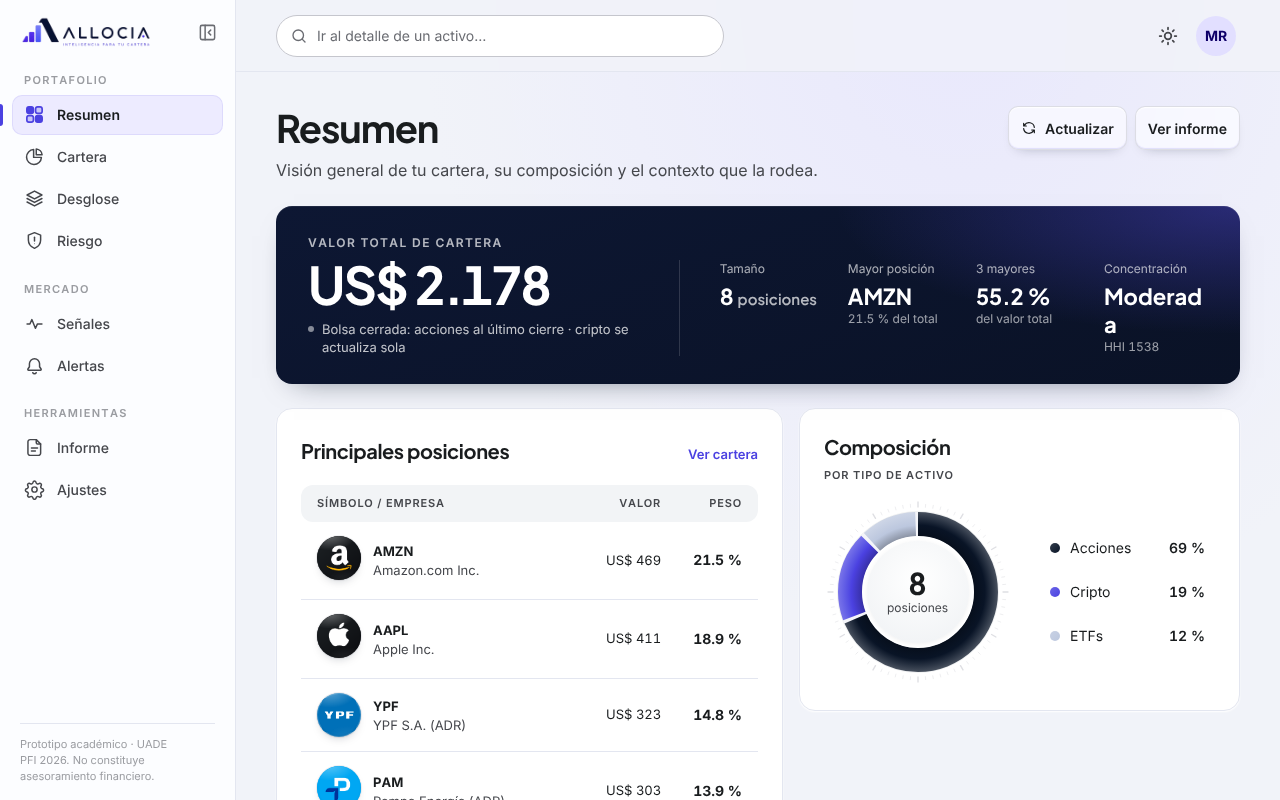
\includegraphics[width=0.82\textwidth]{figures/pantallas/web/w-01-resumen.png}\\[6pt]
	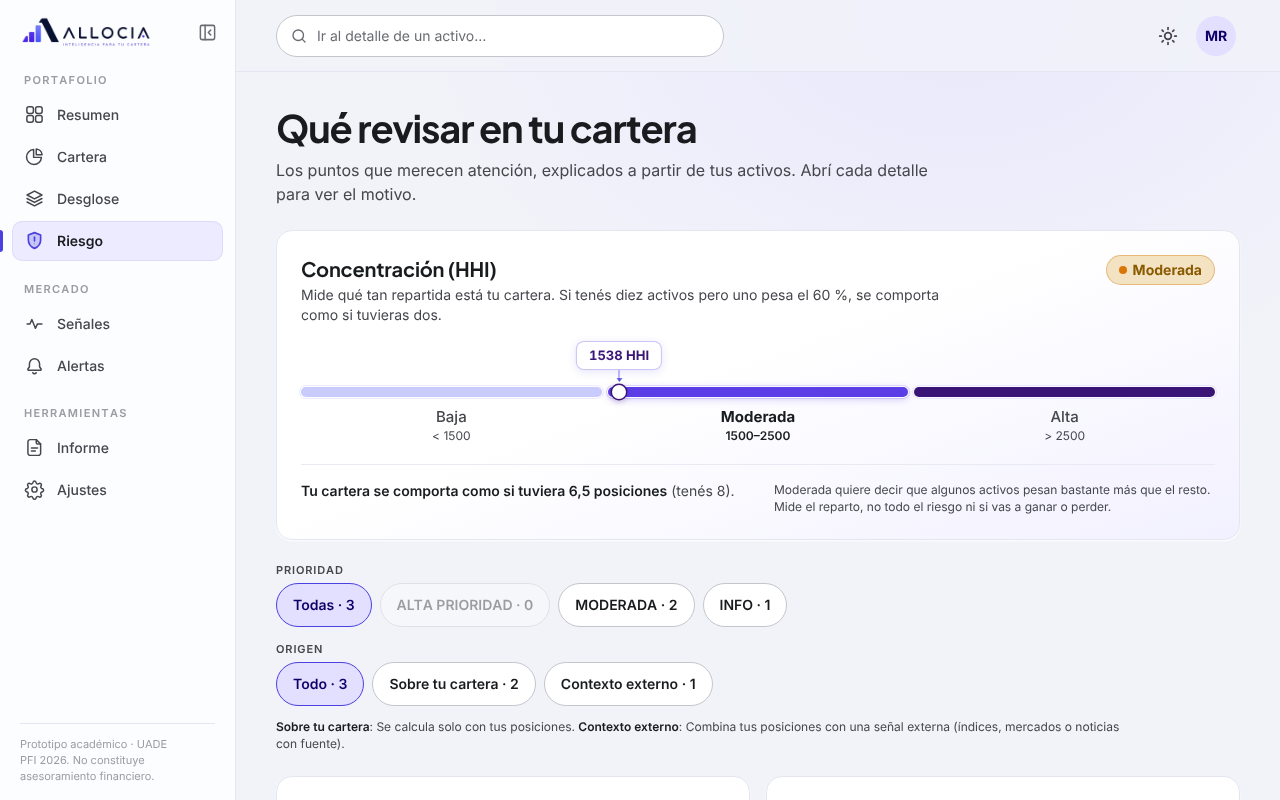
\includegraphics[width=0.82\textwidth]{figures/pantallas/web/w-03-riesgo.png}
	\caption{Capturas del cliente web: Resumen y Riesgo, con una cuenta de prueba. Fuente: elaboración propia.}\label{fig:pant-web}
\end{figure}

La Figura~\ref{fig:pant-web2} presenta Cartera y Señales. En Cartera, el usuario agrega un activo con su ticker y su cantidad, y el sistema lo clasifica por clase, sector, región y moneda; cada posición muestra la cantidad, el precio con la fecha del dato, el valor y el peso, y puede editarse o eliminarse. Señales reúne el contexto externo con su fuente, la fecha del dato y la de consulta: el índice GPR con su nivel sobre una escala (bajo, moderado o elevado), el sentimiento del mercado cripto y la dominancia de BTC, entre otras señales.
\begin{figure}[ht]
	\centering
	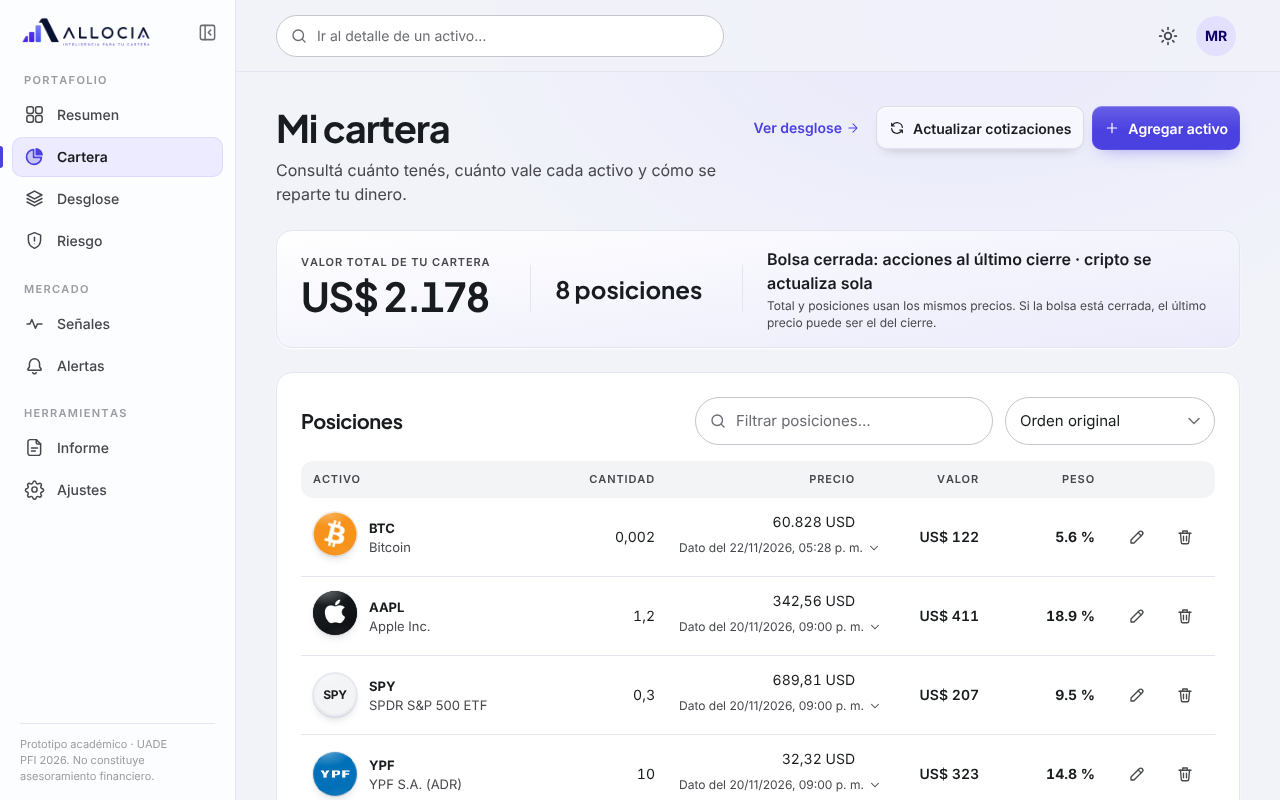
\includegraphics[width=0.82\textwidth]{figures/pantallas/web/w-02-cartera.png}\\[6pt]
	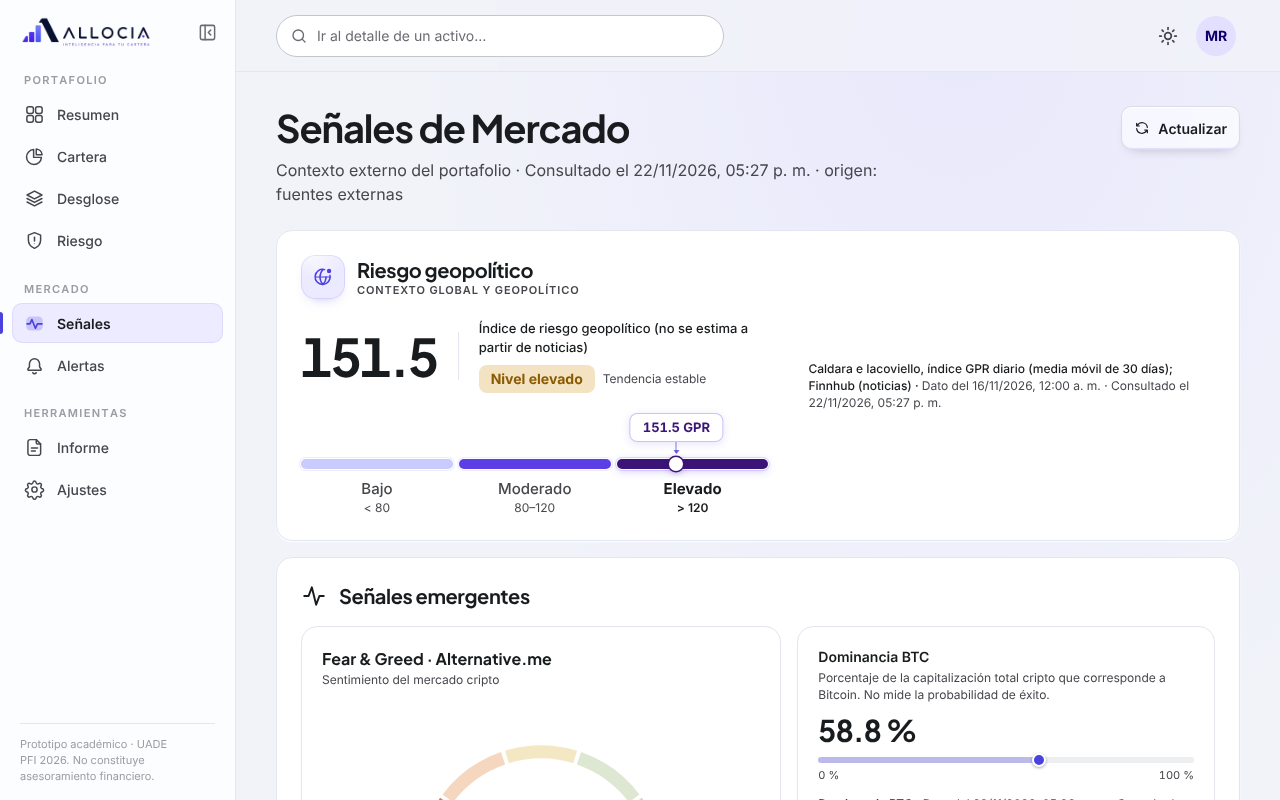
\includegraphics[width=0.82\textwidth]{figures/pantallas/web/w-04-senales.png}
	\caption{Capturas del cliente web: Cartera y Señales, con una cuenta de prueba. Fuente: elaboración propia.}\label{fig:pant-web2}
\end{figure}

La Figura~\ref{fig:pant-movil1} muestra las pantallas de Resumen, Señales y Riesgo de la aplicación móvil, y la Figura~\ref{fig:pant-movil2} las observaciones con su origen y la regla aplicada, la carga de posiciones en Cartera y Ajustes, con la cuenta de demostración y su portafolio cargado.
\begin{figure}[ht]
	\centering
	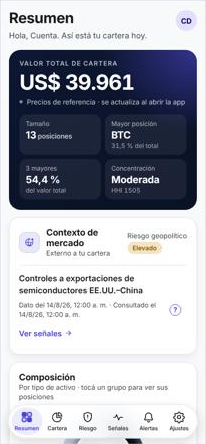
\includegraphics[height=7.4cm]{figures/pantallas/ez-01-resumen.png}
	\hspace{0.3cm}
	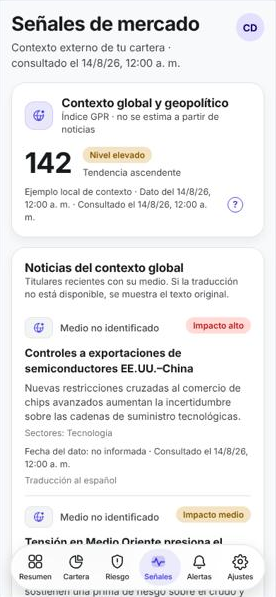
\includegraphics[height=7.4cm]{figures/pantallas/ez-05-senales.png}
	\hspace{0.3cm}
	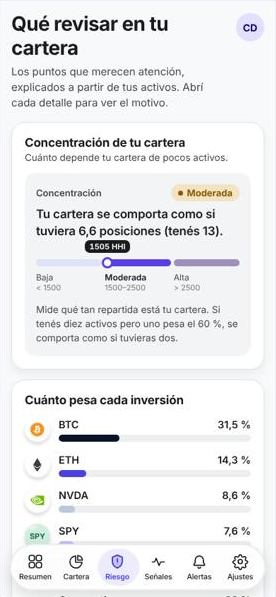
\includegraphics[height=7.4cm]{figures/pantallas/ez-03-riesgo.png}
	\caption{Capturas del prototipo móvil: Resumen, Señales y Riesgo. Fuente: elaboración propia.}\label{fig:pant-movil1}
\end{figure}
\begin{figure}[ht]
	\centering
	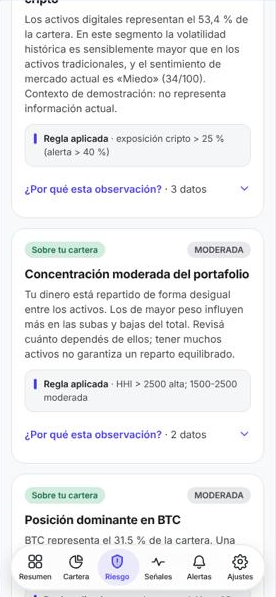
\includegraphics[height=7.4cm]{figures/pantallas/ez-04-riesgo-evidencia.png}
	\hspace{0.3cm}
	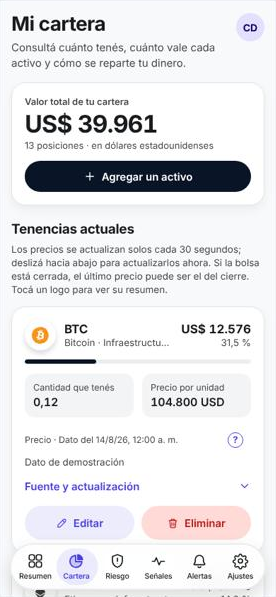
\includegraphics[height=7.4cm]{figures/pantallas/ez-02-cartera.png}
	\hspace{0.3cm}
	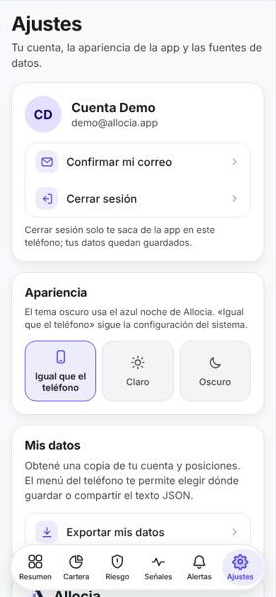
\includegraphics[height=7.4cm]{figures/pantallas/ez-06-ajustes.png}
	\caption{Capturas del prototipo móvil: observaciones con su regla aplicada, Cartera y Ajustes. Fuente: elaboración propia.}\label{fig:pant-movil2}
\end{figure}

Las capturas documentan un estado del prototipo, no la vigencia de las señales ni el cumplimiento de todos los requerimientos. Un indicador de origen global puede ocultar que algunas señales son locales; por eso RF5 pide la procedencia por componente. La baja de cuenta está implementada y probada (Subsubsección~\ref{sec:reverificacion-octubre13}), aunque las capturas móviles no incluyen esa pantalla; la política de privacidad y la pantalla de baja se muestran en el Anexo~\ref{annex:wireframes}.

\FloatBarrier
\section{Tecnologías utilizadas}\label{sec:tecnologias}

React Native con Expo implementa el cliente móvil: una base de código en TypeScript produce las aplicaciones de iOS y Android y simplifica la generación de instaladores con EAS Build. Next.js implementa el cliente web; su servidor intermedio recibe el token en una cookie \texttt{HttpOnly} y reenvía las solicitudes a la API, de modo que el navegador no maneja la credencial. TypeScript permite describir los contratos compartidos entre la API y los clientes y detectar incompatibilidades al compilar. NestJS organiza el backend en módulos con responsabilidades separadas (identidad, portafolio, señales, observaciones e informes), lo que permite probar cada uno por separado (RNF6). PostgreSQL, con TypeORM como capa de acceso, aporta integridad referencial: la clave foránea obligatoria entre posición y usuario, con eliminación en cascada, impide posiciones huérfanas. Redis aporta la caché de señales con tiempo de vida y el contador compartido del límite de solicitudes entre instancias. Vercel y Railway publican el cliente web y la API a partir del repositorio, sin infraestructura propia. La elección de TypeScript en todas las capas favorece una base tecnológica común para el equipo y la separación entre interfaz y reglas.

Los datos externos provienen de Alternative.me (índice Fear \& Greed), CoinGecko (cotizaciones y dominancia de Bitcoin), Finnhub (cotizaciones y noticias), DefiLlama (valor total bloqueado), Polymarket (probabilidades de mercados de predicción), FRED, la base de datos económica de la Reserva Federal de St. Louis, y la planilla diaria del índice GPR que publican Caldara e Iacoviello \parencite{CaldaraIacoviello2022}. Anthropic provee el modelo de lenguaje de los informes por activo y Resend el envío de correo transaccional.

La capa explicable es un motor de condiciones escritas en TypeScript, sin llamadas a un modelo de lenguaje. Reglas y métricas forman una explicación inspeccionable; su utilidad depende de que el usuario comprenda los términos y los límites del cálculo. Los informes por activo son una capa distinta, que sí usa un modelo de lenguaje (Subsección~\ref{sec:seguridad}).

\section{Implementación y reglas}\label{sec:implementacion}

El análisis multiplica la cantidad por el precio del instrumento (el de referencia del catálogo o, en el servicio publicado, la cotización verificada de la Subsección~\ref{sec:integracion-fuentes}), suma valores y normaliza pesos. La clasificación procede del catálogo. Se calculan HHI, número efectivo de posiciones, mayor posición y peso conjunto de las tres mayores posiciones. La cartera vacía se trata como ausencia de exposición, no como una cartera óptimamente diversificada.

La Tabla~\ref{tab:umbrales} documenta las condiciones del código. Los porcentajes se refieren al valor de la cartera. Los umbrales son heurísticas del prototipo, no límites regulatorios ni recomendaciones de inversión.
\begin{table}[ht]
\centering\small
\caption{Condiciones de concentración del motor. Fuente: elaboración propia a partir del código.}\label{tab:umbrales}
\begin{tabular}{p{4cm}p{8.2cm}}\hline
\textbf{Indicador} & \textbf{Condición documentada}\\\hline
HHI & Baja: $HHI\leq1500$; moderada: $1500<HHI\leq2500$; alta: $HHI>2500$.\\
Mayor posición & Observación si su peso supera el 25\,\%.\\
Tres mayores posiciones & Observación si suman más del 60\,\% y hay más de tres posiciones.\\
Criptoactivos & Atención por encima del 25\,\%; alerta por encima del 40\,\%.\\
Tecnología & Condición de concentración sectorial por encima del 35\,\%.\\
Argentina & Condición de exposición regional por encima del 10\,\%.\\\hline
\end{tabular}
\end{table}

Las reglas de contexto añaden condiciones específicas. Entre ellas, una exposición energética superior al 5\,\% junto con un evento relacionado, una probabilidad de evento de tasas superior al 55\,\% y una probabilidad de recesión superior al 20\,\% combinada con menos del 5\,\% en stablecoins. Su interpretación es heurística: una stablecoin, por ejemplo, no es necesariamente un activo libre de riesgo. La evidencia de cada observación permite revisar esas condiciones y sus supuestos.

Los escenarios publicados se construyen a partir de informes recientes con hechos y fuentes verificables. Cada escenario presenta una condición, una dirección posible y su explicación. Se retiran las variaciones porcentuales fijas por clase de activo de la versión inicial. Cuando el respaldo es insuficiente, se informa la ausencia de escenarios en lugar de completarlos con porcentajes o probabilidades inventadas.

\section{Integración de fuentes de datos}\label{sec:integracion-fuentes}

En desarrollo, el servicio de señales mantiene el conjunto de demostración usado para validar las reglas iniciales. En producción se excluyen esos valores y se publican señales externas con su disponibilidad indicada. La capa de integración consulta cotizaciones y noticias generales, por empresa y cripto; limita tiempos y tamaño de respuesta, acepta solo URLs HTTPS y descarta fechas futuras o más antiguas que el umbral. Si falta cobertura o una cotización verificable, la valuación productiva se rechaza en vez de recurrir al precio de demostración.

Cada componente lleva fuente, condición (externa o de demostración) y fecha del dato; en las consultas externas se agrega la fecha de consulta. Si el proveedor no informa la fecha del dato, se muestra esa ausencia en lugar de la fecha actual. El conjunto se identifica como mixto cuando una consulta externa tiene éxito y otros componentes siguen siendo locales. Se rechazan valores de Fear \& Greed y dominancia fuera de 0--100, y el TTL de caché se distingue de la antigüedad del dato original. La Sección~\ref{chap:pruebas} registra pruebas controladas y consultas reales. La Figura~\ref{fig:flujo-informacion} muestra el recorrido de la información desde cada proveedor hasta el usuario y el estado de cada componente. El índice GPR se obtiene de la planilla diaria pública de sus autores: la API descarga el archivo con límites de tiempo y tamaño, toma la última fila válida, usa la media móvil de 30 días como valor de referencia para evitar el ruido de un solo día, clasifica el nivel (bajo por debajo de 80, moderado entre 80 y 120, elevado por encima de 120) y la tendencia (media de 7 días frente a la de 30), descarta lecturas con más de 21 días o con fecha futura y conserva el resultado en caché durante seis horas. La fecha que se muestra es la del último día publicado, no la de la consulta.
% Infografía: recorrido de la información desde las fuentes externas hasta el usuario,
% con el estado de cada componente en el prototipo.
\begin{figure}[ht]\centering
\begin{tikzpicture}[
  font=\scriptsize,
  src/.style={draw,rounded corners,align=left,text width=3.4cm,inner sep=3pt,minimum height=0.55cm},
  live/.style={src,fill=green!10},
  demo/.style={src,fill=orange!12},
  plan/.style={src,fill=black!6,draw=black!50,dashed},
  unv/.style={src,fill=yellow!18},
  stage/.style={draw,rounded corners,align=center,text width=3.6cm,inner sep=4pt,minimum height=1.05cm,fill=blue!5},
  arr/.style={-{Stealth},thick}]
% Columna 1: fuentes externas
\node[live] (f1) {Finnhub: cotizaciones y noticias de acciones};
\node[live,below=0.18cm of f1] (f2) {CoinGecko: precios y dominancia BTC};
\node[live,below=0.18cm of f2] (f3) {Alternative.me: Fear \& Greed};
\node[live,below=0.18cm of f3] (f4) {FRED: series macroeconómicas};
\node[live,below=0.18cm of f4] (f5b) {DefiLlama (TVL) y Polymarket (precios implícitos): consulta registrada el 22/10};
\node[live,below=0.18cm of f5b] (f5) {Caldara e Iacoviello: índice GPR diario (planilla pública)};
\node[plan,below=0.18cm of f5] (f6) {Notificaciones push en el navegador: previstas};
\node[above=0.25cm of f1,font=\footnotesize\bfseries] {Fuentes externas};
% Columna 2: API
\node[stage,right=1.0cm of f2,yshift=-0.2cm] (a1) {\textbf{Normalización y procedencia}\\fuente, fecha del dato, fecha de consulta, estado en vivo / demostración};
\node[stage,below=0.3cm of a1] (a2) {\textbf{Caché de señales}\\Redis, 15 minutos; no prolonga la vigencia del dato};
\node[stage,below=0.3cm of a2,fill=green!8] (a3) {\textbf{Motor de reglas}\\determinista: pesos, HHI, umbrales de la Tabla~\ref{tab:umbrales}};
\node[stage,below=0.3cm of a3,fill=purple!8] (a4) {\textbf{Capa de informes con modelo de lenguaje}\\snapshot público, sin cartera; esquema y citas validados};
\node[above=0.25cm of a1,font=\footnotesize\bfseries] {API (NestJS)};
% Columna 3: clientes y usuario
\node[stage,right=1.0cm of a2,text width=2.6cm] (c1) {\textbf{Cliente web}\\computadora o navegador del teléfono};
\node[stage,below=0.3cm of c1,text width=2.6cm] (c2) {\textbf{Aplicación móvil}\\iOS y Android, misma cuenta};
\node[draw,rounded corners,align=center,text width=2.6cm,inner sep=4pt,fill=blue!12,below=0.5cm of c2] (u) {\textbf{Usuario}\\observación, evidencia y escenarios con fuentes};
\node[above=0.25cm of c1,font=\footnotesize\bfseries] {Presentación};
% Flechas
\foreach \f in {f1,f2,f3,f4,f5b,f5}\draw[arr,black!60] (\f.east)--(a1.west);
\draw[arr,black!40,dashed] (f6.east)--(a1.west);
\draw[arr] (a1)--(a2);\draw[arr] (a2)--(a3);\draw[arr] (a1.east) to[out=0,in=180] (c1.west);
\draw[arr] (a3.east) to[out=0,in=180] (c2.west);\draw[arr] (a4.east) to[out=0,in=180] (c2.west);
\draw[arr] (a3.east) to[out=0,in=180] (c1.west);\draw[arr] (a4.east) to[out=0,in=180] (c1.west);
\draw[arr] (c1)--(c2);\draw[arr] (c2)--(u);
\draw[arr] (a1.south east) to[out=-60,in=120] (a4.north east);
% Leyenda
\node[demo,text width=2.1cm,below=0.55cm of a4] (l2) {Demostración local (solo desarrollo)};
\node[live,text width=2.1cm,left=0.15cm of l2] (l1) {Consulta externa verificada};
\node[plan,text width=2.1cm,right=0.15cm of l2] (l3) {Previsto, no implementado};
\end{tikzpicture}
\caption{Recorrido de la información desde las fuentes hasta el usuario. Fuente: elaboración propia.}\label{fig:flujo-informacion}
\end{figure}


\section{Seguridad, privacidad y límites de la IA}\label{sec:seguridad}

La API dispone de registro e inicio de sesión, JWT de siete días (604800 segundos), versión revocable por cuenta y hash bcrypt con factor 12. La web recibe el token solo en una cookie \texttt{HttpOnly}, \texttt{SameSite=Strict}; el cliente móvil lo guarda en SecureStore. El guard verifica firma, emisor, audiencia, vencimiento, cuenta y versión. El backend agrega CORS con orígenes declarados, validación de origen para mutaciones con cookie, límites de cuerpo y solicitudes, cabeceras de seguridad y errores internos sin detalles. Redis es obligatorio en producción para compartir el límite entre instancias.

Las cantidades se cifran en la aplicación con AES-256-GCM, IV aleatorio y autenticación antes de persistirse. La clave es obligatoria al iniciar en producción y no se comparte con el proveedor de IA. La migración cifra las cantidades previas y solo se aplica con una copia de seguridad restaurable. La pantalla Cuenta permite exportar y eliminar datos; la baja borra por cascada posiciones, alertas y dispositivos. El ensayo de restauración de una copia cifrada y la verificación TLS de PostgreSQL se describen en la Subsección~\ref{sec:regresion-integrada}; la recuperación completa del servicio y la retención productiva quedan fuera de lo evaluado.

Nombre, correo y posiciones vinculadas a una cuenta son datos personales alcanzados por la Ley 25.326 (Subsubsección~\ref{subsec:marco-normativo}). El diseño traduce sus exigencias en RF9, RF10 y RNF9: aviso previo, consentimiento registrado, exportación y baja de cuenta. El envío de un snapshot público del activo, sin identidad ni cantidades, al proveedor del modelo de lenguaje responde a la restricción sobre transferencias internacionales. Los proveedores de alojamiento, correo y modelo (Vercel, Railway, Resend y Anthropic) operan desde el exterior: el nombre, el correo y las cantidades cifradas de una cuenta pueden alojarse o circular fuera del país, de modo que la evaluación del artículo 12 no se limita al proveedor del modelo. El uso con datos reales exige definir antes el responsable, los plazos de conservación y el canal de derechos, evaluar formalmente esas transferencias y analizar con asesoramiento legal la inscripción de la base de datos ante la autoridad de control.

Frente al régimen del mercado de capitales (Subsubsección~\ref{subsec:marco-normativo}), Allocia no está inscripta como agente ante la CNV ni emplea idóneos: se define como herramienta de análisis que no presta asesoramiento habitual y profesional, no interviene en la oferta pública ni ejecuta operaciones, y lo informa en sus avisos (RNF8 y RNF10). Por analogía adopta el lenguaje comprensible y la explicación de cada observación como criterios de diseño. El encuadre depende del funcionamiento efectivo del servicio y no de un aviso de finalidad académica; una apertura pública con recomendaciones personalizadas obligaría a revisarlo con asesoramiento legal.

La implementación integra Anthropic mediante una clave exclusiva del backend y un modelo configurado por entorno. El modelo recibe un snapshot público del activo, no identidad ni cantidades. Titulares y noticias se marcan como datos no confiables; el prompt prohíbe obedecer instrucciones embebidas y el modelo no dispone de herramientas para operar o alterar posiciones. La salida se valida con un esquema: las referencias deben pertenecer al snapshot y cada cita factual debe coincidir literalmente con su fuente. Ante datos ausentes, fuente vieja, respuesta inválida o proveedor sin configurar, el informe se abstiene y no crea alertas. Estas medidas reducen el riesgo de inyección y de alucinación, aunque no lo eliminan \parencite{OWASPPromptInjection}.

La inyección de \textit{prompts} es el riesgo principal de las aplicaciones con modelos de lenguaje según OWASP; en su variante indirecta, contenido recuperado de fuentes externas altera el comportamiento del modelo sin que el atacante use la interfaz \parencite{OWASP2025llm,Greshake2023indirect}. El mismo vector figura entre los riesgos propios de la IA generativa, para los que se recomiendan pruebas adversariales (\textit{red-teaming}) que evalúen la resiliencia \parencite{NIST2024genai}. Titulares de noticias y de mercados de predicción son exactamente ese tipo de contenido. Las mitigaciones aplicadas siguen las estrategias de OWASP: segregar y etiquetar el contenido externo como no confiable, restringir el rol del modelo en la instrucción de sistema, validar la salida con un esquema y con código determinista, negar al modelo funciones de escritura y mantener la decisión en la persona. Los reguladores de valores agregan la dependencia de proveedores externos de modelos y datos como riesgo de concentración \parencite{IOSCO2025ai}; en Allocia el proveedor es sustituible por configuración y el motor de reglas no depende de él.

La gestión de estos riesgos se organiza en cuatro funciones \parencite{NIST2023airmf}: gobernar (responsables y política de uso del modelo), mapear (contexto, usuarios afectados y componentes de terceros), medir (casos de seguridad e IA de la Subsección~\ref{sec:pruebas-produccion}) y gestionar (abstención, registro y corrección de defectos). La Tabla~\ref{tab:controles} resume los controles y su estado.

\begin{table}[ht]
\centering\small\renewcommand{\arraystretch}{1.15}
\caption{Controles de seguridad, privacidad e IA y su estado. Fuente: elaboración propia.}\label{tab:controles}
\begin{tabular}{>{\raggedright\arraybackslash}p{5.6cm}>{\raggedright\arraybackslash}p{1.9cm}>{\raggedright\arraybackslash}p{6.1cm}}\hline
\textbf{Control} & \textbf{Estado} & \textbf{Referencia y límite}\\\hline
Autenticación JWT con emisor, audiencia, vencimiento y versión revocable & Aplicado & RNF4; casos SEC del Anexo~\ref{annex:casos-prueba}.\\
Autorización por propietario de posiciones y clave foránea en cascada & Aplicado & RNF4; IT06, IT10 e IT12 con dos cuentas.\\
Contraseñas con bcrypt (factor 12) y recuperación con tokens de un solo uso & Aplicado & RNF5; Subsección~\ref{sec:correo-cuenta}.\\
Cifrado de cantidades (AES-256-GCM) y secretos fuera del repositorio & Aplicado & RNF5; cifrado en reposo del proveedor no acreditado.\\
HTTPS, cookie \texttt{HttpOnly} y \texttt{SameSite=Strict}, CORS y límites de solicitudes & Aplicado & Comprobaciones web adicionales de la Subsubsección~\ref{sec:reverificacion-octubre13}.\\
Aviso de privacidad, consentimiento, exportación y baja de cuenta & Aplicado & RF9, RF10 y RNF9; Ley 25.326, artículos 4 a 6, 14 y 16.\\
Responsable, plazos de conservación y canal formal de derechos & No aplicado & Requisito previo al uso con datos reales.\\
Contenido externo marcado como no confiable y modelo sin funciones de escritura & Aplicado & OWASP LLM01 y LLM06; casos de IA de la Subsección~\ref{sec:pruebas-produccion}.\\
Validación de esquema y de citas literales; abstención ante datos insuficientes & Aplicado & OWASP LLM05 y LLM09; RF11.\\
Snapshot público sin identidad ni cantidades al proveedor del modelo & Aplicado & Ley 25.326, artículo 12; OWASP LLM02.\\
Pruebas adversariales sistemáticas (\textit{red-teaming}) del flujo con modelo & Parcial & Casos de inyección controlados; sin campaña adversarial completa.\\
Etiquetado en la interfaz de contenido por reglas frente a contenido redactado por el modelo & Parcial & RNF10; aviso en Ajustes y en informes, sin evaluación con usuarios.\\
Transferencia internacional a los proveedores de alojamiento, correo y modelo & No aplicado & Ley 25.326, artículo 12; evaluación formal previa al uso con datos reales.\\
Inscripción de la base de datos ante la autoridad de control & No aplicado & Ley 25.326, artículos 3 y 21; requiere asesoramiento legal.\\
Auditoría de seguridad independiente y pruebas de carga & No aplicado & Fuera del alcance del Proyecto.\\\hline
\end{tabular}
\end{table}

\section{Recuperación de acceso y protección de la sesión}\label{sec:correo-cuenta}\label{sec:mejoras-octubre}

El backend integra Resend para recuperar la contraseña y verificar la dirección de correo. Usa tokens aleatorios de un solo uso, almacena su hash y cifra la copia temporal que necesita el envío. Los enlaces caducan y no exponen el token en la ruta consultada al servidor web. La recuperación revoca las sesiones anteriores. Un proceso de envío controla reintentos y utiliza una clave de idempotencia; la respuesta de solicitud es genérica para no revelar si una cuenta existe. La habilitación externa necesita un remitente de un dominio verificado y el origen HTTPS de la web.

La revisión del 10 de octubre agrega un botón para mostrar la contraseña en inicio de sesión y registro; la contraseña aparece oculta por defecto. Las nuevas sesiones duran siete días; cerrar sesión, recuperar la contraseña o eliminar la cuenta siguen revocando las sesiones anteriores. Los tokens emitidos antes mantienen su vencimiento original.

El cliente móvil utiliza autenticación local del sistema operativo mediante Face ID o huella, según el equipo. Después de ingresar con contraseña se permite el acceso; al restaurar una sesión guardada o volver desde segundo plano se pide el desbloqueo. La cancelación y el error mantienen oculta la cartera. Si no hay biometría configurada, se ofrece ingresar con contraseña. La aplicación no recibe ni almacena plantillas biométricas. Este bloqueo local complementa la autorización del servidor: un token vencido sigue vencido y el aislamiento entre cuentas se mantiene en la API.

Se ocultan las vistas privadas mientras la aplicación está inactiva. Se rechazan resultados de autenticación que llegan después de enviar la aplicación al fondo. Las pruebas de esa lógica utilizan un módulo biométrico simulado; la validación física de Face ID y huella se registra en la Subsubsección~\ref{sec:confirmacion-fisica}. La restauración distingue una sesión rechazada de una falla transitoria de red: esta última mantiene el token en SecureStore, ofrece reintentar y no muestra la cartera hasta validar la cuenta.

La navegación utiliza iconos vectoriales asociados a cada sección, áreas táctiles ampliadas y márgenes seguros. Las transiciones y la confirmación de acciones respetan la preferencia de movimiento reducido. Los informes se presentan en la misma tarjeta que su alerta, con un resumen y detalles desplegables. Las noticias se traducen al español conservando fuente y fecha. Los gráficos representan composición, variaciones e indicadores disponibles; una distribución de cartera o un indicador técnico no se rotula como probabilidad de ganancia.

\section{Actualización de cotizaciones y ejecución de informes}\label{sec:actualizacion-operativa}

La cartera y su total se calculan con las mismas cotizaciones en cada respuesta. Los clientes consultan periódicamente mientras están visibles, con un intervalo de 30 segundos. La caché de precios públicos dura 30 segundos y comparte solicitudes concurrentes. La actualización manual permite consultar nuevamente al proveedor; las pulsaciones repetidas dentro de cinco segundos se agrupan. Esta política reduce solicitudes duplicadas y no altera la demora propia de cada dato.

Se distinguen la fecha informada por el proveedor y la hora de consulta. Un precio de cierre puede conservar la fecha del día anterior aunque la consulta sea reciente. Las criptomonedas pueden modificar la valuación durante un fin de semana mientras las acciones mantienen el último precio informado. Si la fuente falla o la cotización supera los límites admitidos, no se utiliza un precio de demostración ni se presenta el dato como actual. La API guarda una instantánea privada de valuación por usuario, con identificador y hora, durante un máximo de 30 segundos y sin prolongar la vigencia de los precios consultados. Cartera, análisis y reglas reutilizan ese resultado en la misma instancia. Las tenencias se vuelven a leer en cada consulta: una modificación invalida su reutilización. La actualización manual recalcula y un fallo elimina la instantánea. Las respuestas son copias independientes; pasada la ventana, o entre múltiples réplicas de API, dos consultas pueden diferir.

El proceso automático consulta un calendario de sesiones y programa análisis 15 minutos antes de apertura y cierre. La configuración publicada cubre NYSE/Nasdaq durante el período documentado de octubre a diciembre de 2026; necesita mantenimiento y ampliación para otras bolsas. Para cripto se utilizan dos cortes diarios, a las 00:00 y 12:00 UTC. La opción manual sigue disponible y deduplica por usuario, activo y hora. La respuesta diferencia pedidos en cola, en proceso, completados y fallidos; recibir un pedido no significa que el informe ya exista.

Las alertas internas registran los informes nuevos. La pausa de seis horas se aplica a avisos automáticos repetidos de un mismo activo; un análisis manual puede avisar a su solicitante una vez. La interfaz prioriza informes recientes y evita que alertas antiguas oculten el resultado nuevo. La recepción depende de permisos, dispositivo, conectividad y entrega de los proveedores.

\section{Oportunidades fuera de la cartera}\label{sec:oportunidades}

La ampliación separa las vistas de cartera y oportunidades en web y móvil. Una lista de seguimiento por cuenta permite observar activos no poseídos sin modificar cantidades. La búsqueda devuelve identificación y cotización verificables de Finnhub y CoinGecko; los límites de estos proveedores siguen vigentes. La preferencia de alertas de oportunidades es independiente, comienza desactivada y permite elegir todo el universo cubierto o solo los activos seguidos. Se permiten hasta 50 seguimientos por cuenta; la baja los elimina por cascada y la exportación personal incluye lista y preferencias.

El proceso programado incorpora los activos seguidos al universo configurado y mantiene los cortes regionales y de cripto. La solicitud manual prioriza los seguimientos y revisa hasta 50 activos fuera de las tenencias, deduplicados por cuenta, activo y hora. Rige el límite diario compartido, por lo que la cobertura es parcial y no simultánea para todas las acciones y criptomonedas.

Una oportunidad se publica solo con el último informe del activo, de hasta 24 horas, citas literales validadas, fuentes HTTPS de hasta 48 horas y una suba condicional con evidencia específica. Las noticias generales de cripto no bastan. La cotización se admite como referencia fechada hasta 96 horas en acciones y 30 minutos en cripto. Se muestran condiciones, fuentes, riesgos y escenarios contrarios, sin probabilidades ni rentabilidad garantizada. El push comprueba consentimiento, seguimiento, vigencia e informes posteriores. Las cantidades personales no integran el mensaje ni el contexto del modelo.
